High-order finite element simulations, like MARBL, are becoming more
common as supercomputing architectures continue to become more
heterogeneous.
%
One reason for this is that, by simply adjusting the polynomial order
of the mesh elements, high-order simulations
can tune the FLOPS/byte ratio to optimize performance on a specific architecture.
%
Additionally, high-order finite element methods can improve the overall solution accuracy.
%
Analysis and visualization play a key role in understanding, debugging,
and communicating simulation results, but analysis and visualization frameworks
have traditionally only targeted low-order meshes.
%

The geometry of a high-order data set is traditionally converted
to a low-order approximation using element subdivision, and in order
to maintain the accuracy of the solution, low-order refinement can
in some cases dramatically increase the size of data representation.
%
To make matters worse, the best refinement level is unknown,
and the error propagated by the refinement is not easily understood by users.
%
With the rise of in situ analysis, low-order refinement imposes additional memory
and time constraints on the simulation.
%

\begin{figure}
\centering

\includegraphics[width=0.4\textwidth]{images/dray_crazy}

\includegraphics[width=0.4\textwidth]{images/visit_crazy}
\caption{\label{img:crazy_hex} Two renderings of a single $20^{th}$ order hexahedral element.
On the left, a image rendered by Devil Ray, and on the right, an image rendered
in VisIt by subdividing the element into
9,261 low-order hexahedrons.}
\end{figure}

By default, Ascent performs low-order refines to visualize high-order meshes,
but Ascent has recently integrated Devil Ray~\cite{dray}, a library for natively ray tracing
high-order element meshes.
%
Ascent leverages Devil Ray to provide users an alternative to rendering images via low-order refinement.
%
Fig.~\ref{img:crazy_hex} shows an extreme case of the differences between native support for high-order and element subdivision.
%
The Devil Ray integration in Ascent is a first step in offering native high-order
visualization support to simulations, such as MARBL.


In terms of capability, Devil Ray rendering integrated into Ascent includes
volume plots, pseudocolor plot, mesh plots, isosurfacing and slicing.
%
The Devil Ray plotting capabilities are all image-based.
%
For example, both isosurfacing and slicing are rendered through ray tracing and do not
create actual geometry.
%
Plots can be combined through image compositing.
%

\begin{figure}
\centering
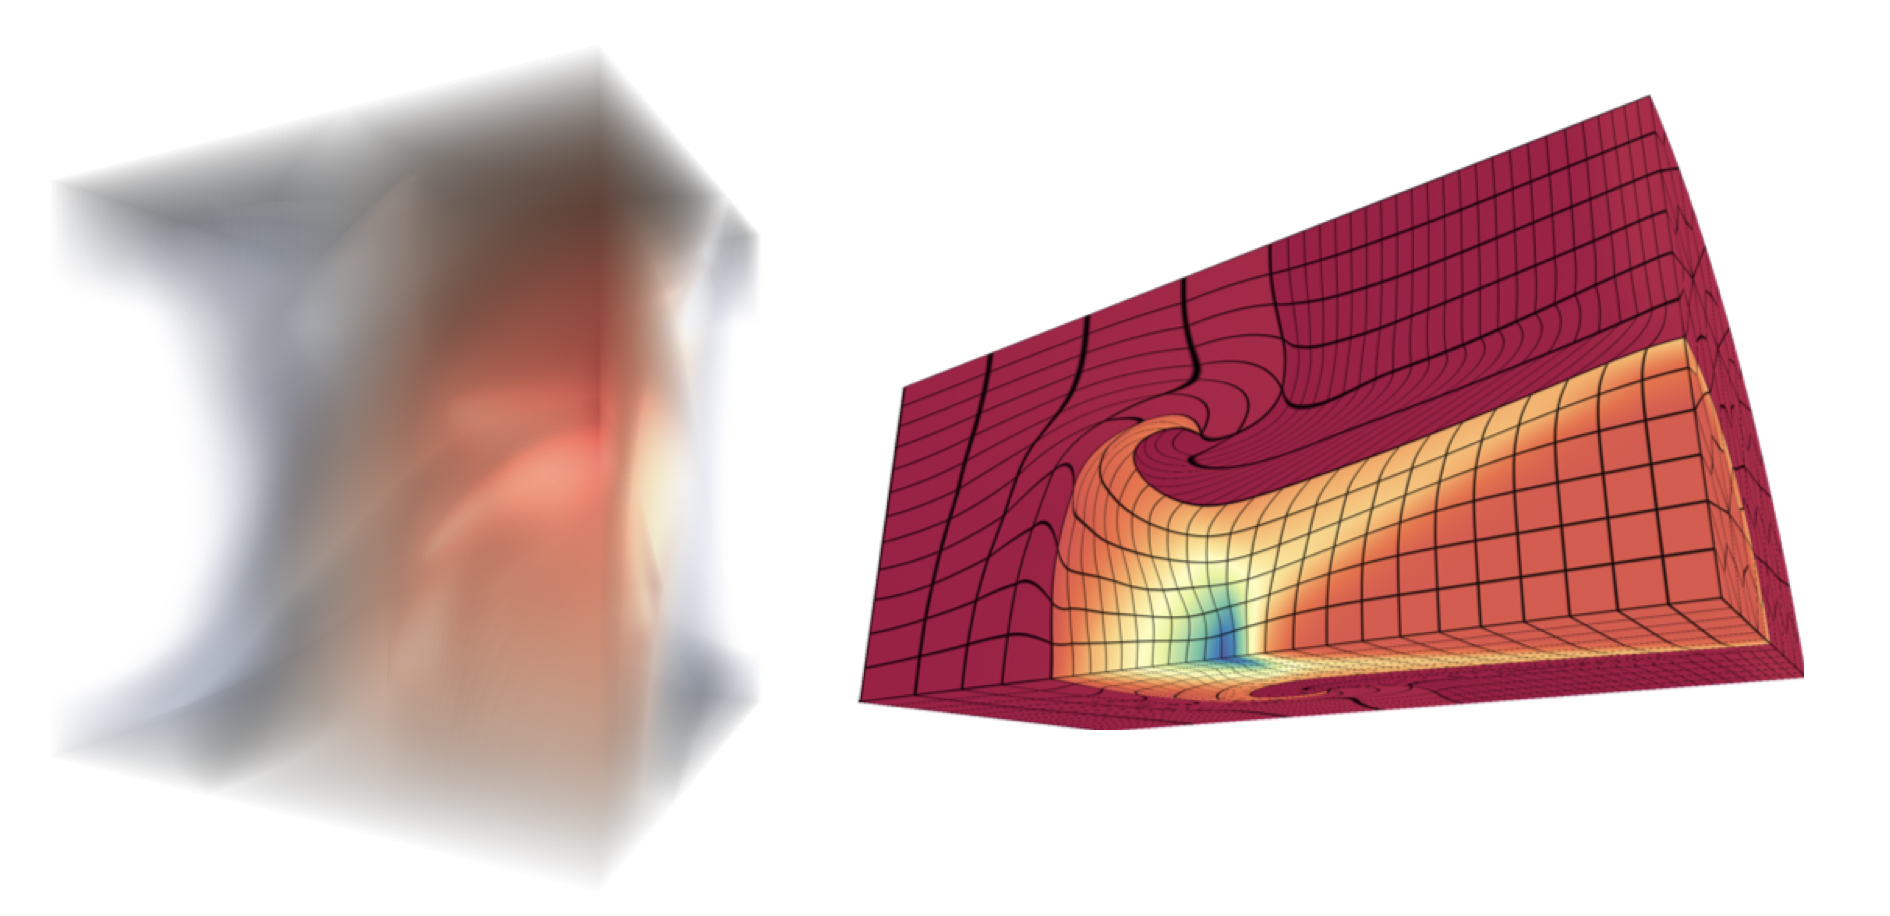
\includegraphics[width=0.8\textwidth]{images/dray_combined}
\caption{\label{img:dray_plots}
Two examples of Devil Ray rendering. On the left, a volume plot of the
Taylor-Green vortex, and on the right, a pseudocolor plot combined with a
volume plot of the triple point problem.}
\end{figure}
